\RequirePackage[l2tabu,orthodox]{nag}
%
    % http://www.tug.org/texlive/Contents/live/texmf-dist/doc/latex/nag/nag.pdf
    % Check for many common mistakes, and give hints on what to use instead.
    % However, always refer to l2tabu for more detailed explanations.
    % Orthodox checks for pitfalls that are not technically incorrect.
    % If you know what you're doing, omit orthodox.
\RequirePackage{pdf14}

\documentclass[12pt,a4paper,british]{article}
\usepackage{etex}
\usepackage{mathptmx}
% \renewcommand{\familydefault}{\rmdefault}
\usepackage[T1]{fontenc}
\usepackage[latin9]{inputenc}
% \usepackage{lmodern}
\usepackage{mathpazo}
\usepackage[protrusion=true,expansion]{microtype}
\usepackage{color,xcolor}
\usepackage{verbatim}
\usepackage{enumitem}
\usepackage{amsmath,amsthm,amsfonts,mathrsfs,bm,mathtools}
\usepackage{graphicx}
\usepackage[a4paper,margin=1.1in]{geometry}
%\geometry{verbose,tmargin=3cm,bmargin=3cm,lmargin=2.5cm,rmargin=2.5cm}
\usepackage{prettyref}
\usepackage[authoryear]{natbib}
\usepackage{booktabs,multirow,multicol,rccol,subfig}
\usepackage{babel}

%############# tikz ######################
\usepackage{todonotes}
    % Use the option "disable" to suppress notes
    % use \missingfigure to locate a place holder for a figure
    % \missingfigure{} has optional text to add
%############# tikz ######################

\usepackage[unicode=true,
			bookmarks=true,
			bookmarksnumbered=true,
			bookmarksopen=false,
			breaklinks=false,
			pdfborder={0 0 1},
			backref=false,
			colorlinks=true]{hyperref}
\hypersetup{final,
			bookmarksopen,
			bookmarksnumbered,
			urlcolor={blue},
			linkcolor={blue},
			citecolor={blue},
			pdfstartview={XYZ null null fitH}}
\pdfminorversion=4
\usepackage{setspace}
\PassOptionsToPackage{nodisplayskipstretch}{setspace}
\onehalfspacing

\ifx\proof\undefined\
  \newenvironment{proof}[1][\proofname]{\par
    \normalfont\topsep6\p@\@plus6\p@\relax
    \trivlist
    \itemindent\parindent
    \item[\hskip\labelsep
          \scshape
      #1]\ignorespaces
  }{%
    \endtrivlist\@endpefalse
  }
  \providecommand{\proofname}{Proof}
\fi


\newlist{casenv}{enumerate}{4}
\setlist[casenv]{leftmargin=*,align=left,widest={iiii}}
\setlist[casenv,1]{label={{\itshape\ \casename} \arabic*.},ref=\arabic*}
\setlist[casenv,2]{label={{\itshape\ \casename} \roman*.},ref=\roman*}
\setlist[casenv,3]{label={{\itshape\ \casename\ \alph*.}},ref=\alph*}
\setlist[casenv,4]{label={{\itshape\ \casename} \arabic*.},ref=\arabic*}

\makeatletter

\providecommand{\casename}{Case}

%%%%%% Theorem env with within section counter %%%%%%
\newtheorem{theorem}{Theorem}[section]
\newtheorem{definition}{Definition}[section]
\newtheorem{assumption}{Assumption}[section]
\newtheorem{prop}{Proposition}[section]
\newtheorem{lemma}{Lemma}[section]

\graphicspath{{graphs/}}


\begin{document}

\title{Productive use of in-vehicle time and its effect for the values of travel time and reliability}

\author{Dereje Abegaz \and Mogens Fosgerau}

\date{\today}

\maketitle

\begin{abstract}
Automated vehicles make it increasingly possible to carry out useful activities while travelling. This paper analyses a commuter's optimal allocation of time among different activities and the implication of a productive use of in-vehicle time on the commuter's valuation of travel time and reliability. We showed the existence of an optimal time allocation. Results in this paper indicate that the value of travel time declines with the productivity of in-vehicle time and that it equals zero if the commuter does not have binding time constraints at home and work. We also discussed the implication of the productive use of time on the willingness to pay for an increase in the degree of automation of the vehicles and other technologies advances that can enhance the productivity of in-vehicle time.
\end{abstract}

\section{Introduction}
\label{sec:introduction}
% by making travel more convenient, more comfortable, or by providing the opportunity to undertake useful economic activity or pleasurable social activity.

% IFT discussion paper [value-saving-travel-time]

In a round-table discussion at ITF, 30 experts from 14 countries identified one of the challenges in the valuation of travel time savings as being the need to account for the quality of travel conditions: The quality component of travel time needs to be incorporated in assessment of the benefits of quicker journey times. The factors that affect the quality of the travel experience include comfort, convenience, frequency, reliability and the possibilities for utilisation of time spent travelling on other activities. In practical terms this means assessing the willingness-to-pay for reduced travel time versus the willingness-to-pay for improvements in travel conditions, and integrating these two assessments in project choice functions (\href{https://www.itf-oecd.org/sites/default/files/docs/value-saving-travel-time.pdf}{Source})

Continued improvements in Information Communication Technology (ITC) and automation, productive use of time ....

Mobile communication devices are transforming the experience of travel, making it possible to work, play games or watch videos while travelling on planes, trains and buses. The car industry promises to free car drivers from driving, thereby enabling an even more drastic transformation of car travel. This paper explores the observation that the new technologies have in common that they make it possible to carry out activities while travelling that substitute for activities elsewhere, at home or at work.

In-vehicle productivity increases when it becomes possible to do things while travelling that were not possible before. This has happened for passengers in trains and buses, who now can use mobile devices  to do new things. It is happening also in planes where internet access during flight is gradually becoming available. Of course, car manufacturers are promising that soon car drivers can be relieved from driving.

This paper looks at the impact of increasing in-vehicle productivity on allocation of commuter's time across different activities and the values of time and reliability. This is of fundamental importance in transport economics and modelling. The values of travel time and reliability are important behavioural quantities as they represent the lion's share of benefits from large infrastructure projects.

We built a model that examines how a commuter optimally allocates his/her time budget among different a activities where some of these activities can only be carried out at home or work. We showed existence of an optimal allocation of time and analysed the optimal scheduling choice in the presence of deterministic and random travel times. We also examined how the values of travel time and reliability change with increasing productivity of in-vehicle time.

Non-work related may include talking on the phone, reading and writing, eating and drinking, planning things, looking through the window, relaxing, watching videos, and work related activities include writing, reading, talking on the phone, planning, video conferencing, etc.

The rest of the paper is organised as follows. The next section sets out the model set up and foundation for the rest of the paper. The third and fourth sections analyse the optimal allocation of time among different activities and the value of travel time, value of reliability and value of headway when trip duration is random or deterministic. The final section provides a summary of our findings and concluding remarks.

\section{The model}
\label{sec:model1}

Consider a commuter who begins a day at home and who has to take a trip to a workplace where he or she finishes the day. The commuter has a time budget of $Q$ time units on the clock interval $[0, Q]$ and intends to allocate this among different activities. We distinguish three set of leisure and work activities based on whether they can be undertaken at home, at work, or in-vehicle. The first set of work and leisure activities include those which the commuter can carry out at home, at work and while travelling. We call these activities \textit{mobile activities}. While the range of activities that can be performed during a trip depends on the degree of automation of the vehicle, it may include talking on the phone, reading and writing, eating and drinking, planning, relaxing, watching videos, etc. The set of other leisure (resp. work) activities that can only be carried out at home (work) is referred to as \emph{home-based activities} (\emph{work-based activities}). While home-based activities include cooking, cleaning and other social activities, work-based activities may include meeting, teaching, conducting laboratory experiments, performing construction work, etc.


Let $0<T<Q$ be the travel time for the commute trip. Setting aside $T$ units of time for the trip, the commuter has $Q-T$ units of time available which he or she can freely allocate among the three activities. We denote by $t_{h}$ and $t_{w}$ the time assigned to the home-based and work-based activities, respectively, such that $0<t_{h}\leq t_{d}$ and $0<t_{w}\leq Q-t_{d}-T$ where $t_d$ is the departure time for the commute trip. Given this,  $T+\left(t_{d}-t_{h}\right)+\left(Q-t_{d}-T-t_{w}\right)$ units of time will be available to carry out the mobile activities.


The commuter has preferences over outcomes from the three activities, and given those preferences, he or she allocates the total time so as to obtain the best result among those available. Suppose a unit of output is produced per unit of time assigned to the home-based or work-based activities while the productivity of time assigned to the mobile activities depends on whether they are undertaken at home, at work, or in-vehicle. Suppose the commuter is fully productive when performing the mobile activity at home or at work but may be less so while travelling. This is controlled by a factor $\alpha \in \left[0, 1\right]$, such that the amount of output per unit time spent in performing the mobile activity is $t_{m} = Q - \left( 1 - \alpha \right) T - t_{h} - t_{w}$. Note the parameter $\alpha$ indicates the productivity of in-vehicle time relative to time at work or at home.

\begin{figure}[ht!]
    \centering
    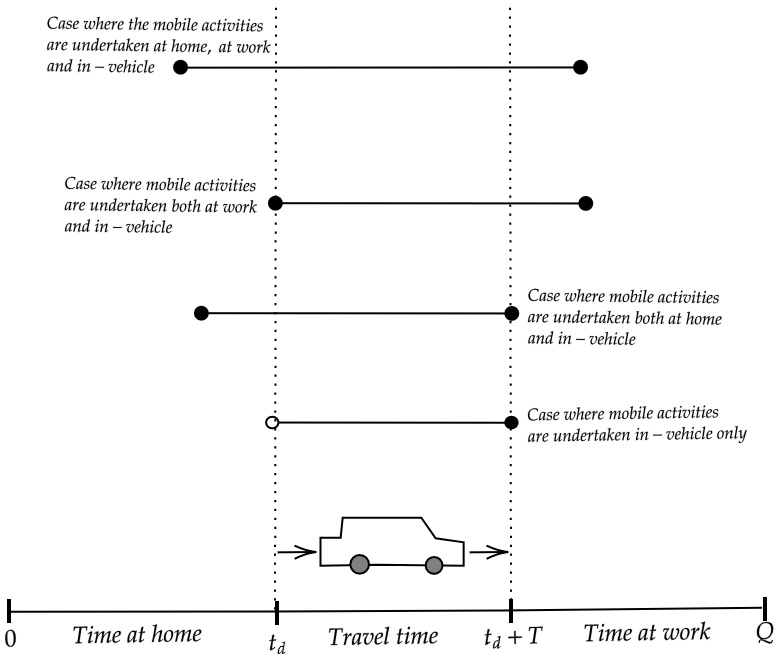
\includegraphics[width=0.5\textheight]{allocationPossibilities.png}
    \caption{Allocation of time with and without binding constraints}
	\label{fig:time_allocation}
\end{figure}

We represent the commuter's preferences by a utility function. The utility of time spent undertaking the home-based activities is given by the function $U_h(t_h)$, which is assumed to be differentiable, increasing and strictly concave. More time assigned to the home-based activities produces more output, so in the limit as $t_h$ approaches 0, $U_h^{\prime}$ is infinity. Similarly, the utility from time assigned to the work-based activities is given by the function $U_w(t_w)$, which has the same property as $U_h(t_h)$. In addition, the utility from time spent in performing the mobile activities is $U_m(t_m)$, which is differentiable, increasing and strictly concave. While $U_m$ depend on the effective units of the mobile activities performed, the latter can be deduced given the total available time and a chosen $\left(t_h, t_w\right)$. As a result, we write $U_m = U_m\left(t_h, t_w\right)$. We assume that $U_{m}^{\prime}\left(0\right) < \infty$ such that the commuter may choose not to carry out any of the mobile activities. Given the above, the commuter's utility function for a given travel time $T$ is%
\begin{equation}
	U\left(t_{h},t_{w};T\right)=U_{h}\left(t_{h}\right)+U_{w}\left(t_{w}\right)+ U_{m}\left(t_{h}, t_{w}\right),
	\label{eq:utility0}
\end{equation} %
where the marginal utility of money is normalised to unity and utility is assumed to be additively separable into different components depending on the activities in which time is spent. 

The model in \eqref{eq:utility0} is similar to that of \citet{Oort1969EvaluationTravellingTime} and  \citet{DeSerpa1971TheoryEconomicsTime}, but compared to them, it accounts for a potential productive use of in-vehicle time and any displeasure from travelling per se as long as it reduces the productivity of in-vehicle time. Further to this, the models by \citet{Becker1965TheoryAllocationTime} and \citet{Johnson1966TravelTimePrice} can be shown to arise as a special case of our model without the mobile activity and where travel time is fully unproductive. 

% The enhanced possibility to under activities in automated vehicles may decrease the dis-utility of travel.

\todo[inline]{May we describe how our model compares against the scheduling model, e.g. \citet{FosgerauEngelson2011ValueTravelTime}}


\begin{definition}
	(\textbf{time allocation}) A time allocation is a pair $\left(t_{h},t_{w}\right)$ where each $0\leq t_{i}\leq Q-T$ indicating a commuter's choice of time allocated to the home-based and work-based activities.
\end{definition}

Given the travel time $T$, the commuter's problem is allocating the $Q-T$ units of time among the home-based, work-based and mobile activities. If $\left(t_{h},t_{w}\right)$ is chosen, then the amount of time available to the mobile activity will be implied by the time budget. Hence, the commuter's problem amounts to choosing $\left(t_{h},t_{w}\right)$ provided that time spent on all activities, including travelling, be within total time budget:
\begin{equation}
t_{h}+t_{w}+T\leq Q.
\label{constraint0}
\end{equation}
This inequality also indicates that some of the time at home and/or at work may be allocated to the mobile activities as illustrated in fig.~\ref{fig:time_allocation}. This depends on whether the commuter has a binding time constraint at home or work. Accordingly, if the commuter faces a binding time constraint both at home and at work, then the mobile activities will be carried out only while travelling. In the absence of binding constraint, however, some of the time at home and/or at work may be assigned to the mobile activities. Given the optimal allocation of time, the commuter will also choose the optimal departure time for the commute trip.


\section{A case with deterministic travel times}

\subsection{The optimal allocation}

If travel time is known with certainty ahead of the trip, the commuter will take this as given and allocate the total time among different activities to maximise utility subject to the constraint that time spent on different activities cannot exceed the total available time:
\begin{align}
\begin{split}
    \max_{t_{h},t_{w}} \, & U\left(t_{h},t_{w};T\right) \\ %& = U_{h} \left(t_{h}\right) +  U_{w}\left(t_{w}\right) + U_{m}\left(t_{h}, t_{w} \right) \\
    \mbox{subject to } \, &  T + t_{h} + t_{w} \leq Q \\
                      \, & t_w, t_h \geq 0
\end{split}
\label{eq:maxProb_fixedT}
\end{align}
That is, given some $T$, $\alpha$, and $Q$, the commuter allocates his or her time in order to maximise utility $U\left( \cdot; T, \alpha, Q \right)$ from among a set of feasible time allocations.

\begin{definition}
(\textbf{feasible time allocation}) A time allocation $\left( t_h, t_w \right)$ is said to be \textbf{\textit{feasible}} if the total time allocated to the home-based and work-based activities does not exceed the commuter's time available for these activities, i.e., $t_h + t_w \leq Q - T$.
\end{definition}

Since the constraint is linear, the set of feasible time allocations is convex. Moreover, the objective function $U$ is strictly concave as it is the sum of strictly concave functions. Thus, \eqref{eq:maxProb_fixedT} is a concave optimisation problem on a convex constraint set. The Lagrangian for the utility maximisation problem can be written as
\begin{equation*}
\mathcal{L} \equiv U\left(t_{h},t_{w};T\right) + \lambda \left(Q - T - t_{h} - t_{w}\right),
\end{equation*}%
where $\lambda$ is a non-negative constant indicating the change in optimal utility following a unit relaxation of the time constraint. The first-order conditions for an optimal allocation $\left(t_h^{\ast}, t_w^{\ast}\right)$ are as follows:
\begin{subequations}
\begin{align}
U_{h}^{\prime}\left(t_{h}^{\ast}\right)-U_{m}^{\prime}\left(t_{h}^{\ast}, t_{w}^{\ast}\right)-\lambda^{\ast} & =0
\label{eq:foc_deterministic_th} \\
U_{w}^{\prime}\left(t_{w}^{\ast}\right)-U_{m}^{\prime}\left(t_{h}^{\ast}, t_{w}^{\ast}\right)-\lambda^{\ast} & = 0
\label{eq:foc_deterministic_tw} \\
\lambda\left(Q - T - t_{h}^{\ast} - t_{w}^{\ast}\right) & =0
\label{eq:foc_deterministic_lmd} \\
\lambda^{\ast},t_{h}^{\ast},t_{w}^{\ast} & \geq 0
\label{eq:foc_deterministic_nonnega}
\end{align}\label{eq:foc_deterministic}
\end{subequations}
These conditions imply that the optimal allocation is characterised by equalisation of the marginal value of time assigned to the home-based and work-based activities, $U_{h}^{\prime}\left( t_{h}^{\ast} \right) = U_{w}^{\prime}\left( t_{w}^{\ast}\right)$. Given $t_{h}^{\ast}$ and $t_{w}^{\ast}$, the effective unit of the mobile activities carried out will be $t_{m}^{\ast} = t_{m}\left( t_{h}^{\ast},t_{w}^{\ast} \right)$. In addition, optimal allocation with binding constraint requires the marginal value of time assigned to the mobile activity be lower than that allocated to each of the home-based or work-based activities. In this case, the difference in the marginal value of time is given by the resource value of time, $\lambda^{\ast}$. If the constraint is non-binding , i.e. $\lambda^{\ast}=0$, then the optimum is characterised by equalisation of the marginal value of time in the three activities. The following theorem establishes existence of an optimum.

\begin{theorem}
\label{thm:optimum_det}
If each $U_{i}\left(\cdot\right)$ is continuous, increasing, twice-continuously differentiable and strictly concave, then there exists a unique optimal allocation $\left( t_{h}^{\ast}, t_{w}^{\ast} \right)$ satisfying the conditions in (\ref{eq:foc_deterministic}).
\end{theorem}

\begin{proof}
Since $\mathcal{L}$ is continuous on a closed interval, by the extreme value theorem, there is an optimal allocation $\left(t_{h}^{\ast},t_{w}^{\ast}\right)$ and a multiplier $\lambda^{\ast}$ at which $\mathcal{L}$ attains maximum. Since the set of feasible time allocations is convex and $U$ is differentiable and strictly concave, the optimal allocation  $\left(t_{h}^{\ast},t_{w}^{\ast}\right)$ and the multiplier $\lambda^{\ast} $ satisfy the first-order conditions in \eqref{eq:foc_deterministic} and that the optimum is unique \citep[Theorem 1.19 and Theorem 1.20 in][]{delaFuente2000MathematicalMethodsModels}.
\end{proof}

Now consider the commuter's choice of departure time in light of the optimal allocation. If the constraint is binding, then time at home and at work will be assigned entirely to the home-based and work-based activities, respectively, with the mobile activities being carried out only while travelling. Hence, at optimum the commuter departs at time $t_{h}^{\ast}$. On the other hand, if the time constraint is non-binding, then the commuter undertakes the mobile activities in-vehicle as well as at home and/or at work. In this case, the optimal departure time may be any time between $t_{h}^{\ast}$ and $Q-t_{w}^{\ast}-T$. 

The utility to an optimising commuter,%
\begin{equation}
U^{\ast}\equiv U\left(t_{h}^{\ast},t_{w}^{\ast};T\right)=\max_{t_{h},t_{w},t_{h}+t_{w}+T\leq Q}U_{h}\left(t_{h}\right)+U_{m}\left(t_{h}, t_{w}\right)+U_{w}\left(t_{w}\right),
\label{eq:UStarDet}
\end{equation}
is defined for a given trip duration and level of productivity of in-vehicle time, hence $t_h^{\ast}= t_h^{\ast} \left(T, \alpha \right)$ and $t_w^{\ast} = t_w^{\ast} \left(T, \alpha \right)$. In the following section, we analyse the welfare effect of a small change in travel time and level of productivity of in-vehicle time.


\subsection{Comparative statics}

\subsubsection*{The effect of productivity enhancement}
An exogenous improvement in the productivity of in-vehicle time is beneficial with the welfare gain from it being proportional to the duration of in-vehicle time and the marginal value of time assigned to the mobile activities:
\begin{equation*}
    \frac{\partial U^{\ast}}{\partial \alpha} = T U^{\prime}_m\left( t_{h}^{\ast}, t_{w}^{\ast} \right) \geq 0.
\end{equation*}
The gain from enhanced productivity is higher with longer travel duration as the marginal benefit spreads across longer duration. This implies that those with longer commute trips will gain more from increased automation and hence will be willing to pay more for an improvement in productivity of in-vehicle time.


\subsubsection*{The value of travel time}
The value of travel time in our model is given by the sum of the resource value of time, $\lambda^{\ast}$, and the marginal gain from performing the mobile activities at work/home as opposed to while travelling:
\begin{equation}
-\frac{\mathrm{d}U^{\ast}}{\mathrm{d}T}  = \left(1 - \alpha\right) U_{m}^{\prime}\left(t_{h}^{\ast}, t_{w}^{\ast}\right) + \lambda^{\ast}.
\label{eq:VOT_det}
\end{equation}
The value of travel time is proportional to $\left(1 - \alpha \right)$ and it is non-negative since $\alpha \in \left[0, 1 \right]$, $\lambda^{\ast} \geq 0$ and $U_{m}^{\prime}\left( \cdot \right) > 0$. Substituting \eqref{eq:foc_deterministic_tw} in \eqref{eq:VOT_det} and rearranging, we have  $-\frac{\mathrm{d}U^{\ast}}{\mathrm{d}T}  = U_{w}^{\prime}\left(t_{w}^{\ast}\right) - \alpha U_{m}^{\prime} \left( t_{h}^{\ast}, t_{w}^{\ast}\right)$. Hence, if travel time is unproductive, i.e., $\alpha=0$, then the value of travel time equals the marginal value of time assigned to the work-based activity. This result was indicated in previous research \citep[e.g.][]{Becker1965TheoryAllocationTime,Johnson1966TravelTimePrice,Oort1969EvaluationTravellingTime,DeSerpa1971TheoryEconomicsTime} with the resulting value of travel time comprising of different elements. For instance, \citet{Becker1965TheoryAllocationTime}  showed that the value of (travel) time is equal to the wage rate while others indicated that the value of reduced (travel) time also includes the subjective value of work \citep{Johnson1966TravelTimePrice}, as time spent at work can be enjoyable, and the value of reduced displeasure \citep{Oort1969EvaluationTravellingTime}, as travelling may be unpleasant. In our model, the marginal value of time assigned to work-based activities equals the sum of the marginal value of time allocated to the mobile activities, $U_m^{\prime} \left(\cdot\right)$, and the resource value of time, $\lambda^{\ast}$. If however $\alpha=1$, then the value of travel time equals just the value of time as a resource. The implication of this is that a unit reduction in travel time will be valued equally as a unit relaxation of the time budget.


\begin{lemma}
If travel time is fully productive and the time constraint is non-binding, then the value of travel time is zero.
\end{lemma}

\begin{proof}
	This follows by substituting $\alpha=1$ and $\lambda^{\ast}=0$ in \eqref{eq:VOT_det}.
\end{proof}
\begin{comment}
	We can see that each of DeSerpa's definitions in fact corresponds to different concepts that had previously appeared in the literature. One of his most interesting comments is related with "leisure", which he defined as the sum of all activities that are assigned more time than is strictly necessary according to the 	new set of constraints. For these activities, the value of saving time is zero, and the value of time allocated to the activity (his "value of time as a commodity") is equal for all such activities and equal to multiplier./., the resource value of time or, what is now evident, to the value of leisure time.
\end{comment}

The result in the above Lemma implies that commuters with non-binding constraint, who have a fully automated vehicle allowing them to perform mobile activities as efficient as they would out of vehicle, will be unwilling to pay for a reduction in travel time. If the constraint is binding, then the value of travel time is positive even if travel time is fully productive. This is so since, in this case, more time is allocated to the mobile activity than desired. 


Compared to previous literature \citep[e.g. ][]{Johnson1966TravelTimePrice,Oort1969EvaluationTravellingTime}, the value of travel time in the current paper includes a potential \textit{loss in value} as a reduction in travel time reduces the time available to productively perform activities while travelling. This was disregarded in previous studies as the possibility of productive use of in-vehicle time was ruled out. Thus, to the extent that the the dis-utility from travel is reflected in reduced productivity of in-vehicle time and the subjective value of time is accounted in $U_w$, the value of travel time in the current study would be lower than implied else the literature. Accounting for the potential productivity of in-vehicle time leads to a lower value of travel time.


\begin{prop}
If a commuter has non-binding time constraint, then his or her value of travel time declines with the productivity of in-vehicle time. On the other hand, if the time constraint is binding, then the value of travel time declines with the productivity of in-vehicle time if the coefficient of relative risk aversion of $U_m$ is less than or equal to unity.
\end{prop}


\begin{proof}
To show this, differentiate \eqref{eq:foc_deterministic_th} and \eqref{eq:foc_deterministic_tw} with respect to $\alpha$ and manipulate to find that $\frac{\partial t_{w}^{\ast}}{\partial\alpha} , \frac{\partial t_{h}^{\ast}}{\partial\alpha} \geq 0$. If the constraint is non-binding, then $\frac{\partial t_{w}^{\ast}}{\partial\alpha}, \frac{\partial t_{w}^{\ast}}{\partial\alpha} > 0$ and $\lambda^{\ast} = 0$. Therefore,%
\begin{equation*}
\frac{\partial\left( - \frac{\mathrm{d}U^{\ast}}{\mathrm{d}T}\right)}{\partial\alpha} = \frac{\left(1 - \alpha\right) T \, U_{h}^{\prime\prime}\left(t_{h}^{\ast}\right) U_{m}^{\prime\prime}\left(t_{h}^{\ast},t_{w}^{\ast} \right)} {U_{h}^{\prime\prime}\left(t_{h}^{\ast}\right) + U_{m}^{\prime\prime}\left(t_{h}^{\ast} t_{w}^{\ast}\right)\left(1+\frac{U_{h}^{\prime\prime}\left(t_{h}^{\ast}\right)}{U_{w}^{\prime\prime}\left(t_{w}^{\ast}\right)}\right)}-U_{m}^{\prime}\left(t_{h}^{\ast}, t_{w}^{\ast}\right) < 0
\end{equation*}
the inequality follows since $U_i^{\prime\prime}\left( \cdot \right) <  0 < U_i^{\prime}\left( \cdot \right)$ and $0\leq \alpha \leq 1$. If however the constraint is binding, then $\frac{\partial t_{h}^{\ast}}{\partial\alpha}=\frac{\partial t_{w}^{\ast}}{\partial\alpha} = 0$, $t_m^{\ast} = \alpha T$, $\frac{\partial t_{m}^{\ast}}{\partial\alpha}=T$ and $\frac{\partial\lambda^{\ast}}{\partial\alpha}=-TU_{m}^{\prime\prime}\left(t_{h}^{\ast}, t_{w}^{\ast}\right)$. Thus,%
\begin{equation*}
\frac{\partial\left(-\frac{\mathrm{d}U^{\ast}}{\mathrm{d}T}\right)}{\partial\alpha}= - U_{m}^{\prime}\left(\alpha T \right) - \alpha T U_{m}^{\prime\prime}\left(\alpha T \right) \leq 0
\end{equation*}
where the inequality holds if $R_m = -\frac{\alpha T U_{m}^{\prime\prime}\left(\alpha T \right)}{U_{m}^{\prime}\left(\alpha T \right)} \leq 1$

\end{proof}

%In general, the effect of a change in the level of productivity of in-vehicle time on the value of travel time is stated in the above proposition.

The result in the above proposition implies that commuters will be willing to pay for increasingly more automated vehicles and other technological advances that make travel more convenient and enhance the possibility to perform useful economic or social activities. While this result has been indicated in empirical studies ({\color{red} e.g., Ducth Value of Time Study}), we derive the result from a behavioural model and showed that it holds in general within the framework of our model.



\subsection{Numerical example}

In this section we illustrate the optimal time allocation, the value of travel time and how the latter changes with respect to the productivity of in-vehicle time based on particular functional forms and parameter values. We consider a commuter with a unit time budget and trip utility:
\begin{align*}
U\left(t_{h},t_{w};T\right) & = \log\left(t_{h}\right) + \frac{1}{2} \log\left(1-\left(1-\alpha\right)T-t_{h}-t_{w}\right)+\log\left(t_{w}\right)
\end{align*}where $0<T<1$. An optimal allocation $\left(t_h^{\ast}, t_w^{\ast}\right)$ is characterised by the following conditions:
\begin{subequations}
	\label{eq:foc_example1}
	\begin{align}
	\frac{1}{t_{h}^{\ast}}-\frac{1}{2\left(1-\left(1-\alpha\right)T-t_{h}^{\ast}-t_{w}^{\ast}\right)}-\lambda^{\ast} & = 0 
	\label{eq:foc_eg1_th} \\
	\frac{1}{t_{w}^{\ast}} - \frac{1}{2\left(1-\left(1-\alpha\right)T - t_{h}^{\ast} - t_{w}^{\ast} \right)} - \lambda^{\ast} & = 0
	\label{eq:foc_eg1_tw}\\
	\lambda\left(1-T-t_{w}^{\ast}-t_{h}^{\ast}\right) & = 0 
	\label{eq:foc_eg1_lamb} \\
	\lambda^{\ast},t_{h}^{\ast},t_{w}^{\ast} & \geq 0.
	\label{eq:foc_eg1_nonnega}
	\end{align}
\end{subequations}
where $\lambda^{\ast} \geq 0$. Whether the time constraint will be active depends on the travel time $T$ and the productivity of in-vehicle time $\alpha$. There are two possibilities: either the constraint is non-binding, and hence the optimal allocation $\left(t_h^{\ast}, t_w^{\ast}\right)$ satisfies $1-(1-\alpha)T - t_h^{\ast} - t_w^{\ast} < 0$, or it is binding, and hence the optimal allocation satisfies $1-(1-\alpha)T - t_h^{\ast} - t_w^{\ast} = 0$. 


\begin{casenv}
	\item If the constraint is non-binding, then the optimal allocation will be the same as that without the constraint. Setting $\lambda^{\ast}=0$ in \eqref{eq:foc_example1}, we obtain the optimal time allocation as $\left( t_{h}^{\ast}, t_{w}^{\ast} \right) = \left(2\frac{1-\left(1 - \alpha \right)T} {5}, 2\frac{1-\left(1 - \alpha \right)T} {5}\right)$. Hence, $t_{m}^{\ast} = \frac{1-\left(1-\alpha\right)T} {5}$ effective units of the mobile activities will be performed at optimum. This means that the total time that will be assigned to the three activities is allocated across them based on the marginal value of time from these activities. The resulting optimal utility is %
	\begin{equation*}
	U^{\ast} = U \left(t_h^{\ast}, t_w^{\ast}\right) = 2\log (2) +  \frac{3}{2}\log\left(\frac{1-\left(1-\alpha\right)T}{5}\right)
	\end{equation*}
	For a given $ \alpha $, the constraint function evaluated at the optimum is $\frac{1-(4\alpha + 1)T}{5}$, thus the constraint is non-binding, i.e., $\lambda^{\ast}=0$ if $T \leq \frac{1}{4\alpha + 1}$.

	The value of travel time is
	\begin{equation*}
	- \frac{\mathrm{d}U^{\ast}}{\mathrm{d}T} = \frac{3}{2} \left( \frac{1-\alpha}{1-\left(1-\alpha\right)T} \right) > 0.
	\end{equation*}
	It achieves its maximum when $\alpha=0$ and declines with the productivity of in-vehicle time:
	\begin{equation*}
		\frac{\partial}{\partial\alpha}\left(-\frac{\mathrm{d}U^{\ast}}{\mathrm{d}T}\right)=-\frac{3}{2\left(1-\left(1-\alpha\right)T\right)} < 0
	\end{equation*} %
	until it equals zero when travel time is fully productive. Notice also that the (absolute) effect of improved productivity is higher at lower productivity levels suggesting potentially higher willingness to pay for the initial transition to automation. 
%	For $\alpha = T = 0.1$, the change in the value of travel time per unit change in productivity of in-vehicle time equals -1.65.

	\begin{figure}[ht!]%
	\centering
	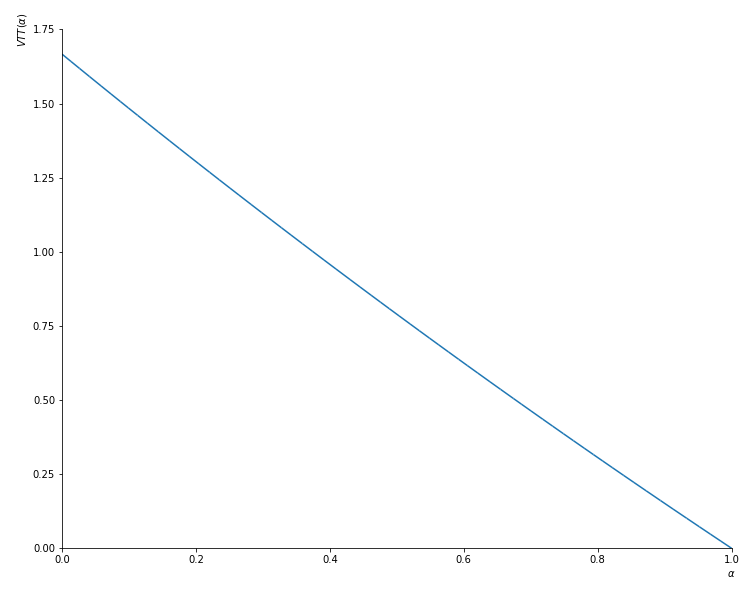
\includegraphics[scale=0.6]{plotNumericalExample02.png}
	\caption{The value of travel time as a function of $\alpha$ for $T=0.1$}%
	\label{fig:example_det}%
	\end{figure}


	\item If the constraint is binding, then all the time at home (resp. work) will be assigned to the home(work)-based activity. Hence, $t_{m}^{\ast}=\alpha T$. Moreover, \eqref{eq:foc_example1} imply that the time available for out-of-vehicle activities, $1-T$, will be allocated equally between the home-based and work-based activities, hence $t_{h}^{\ast}=t_{w}^{\ast}=\frac{1-T}{2}$ and $\lambda^{\ast} = \frac{1-\left(4\alpha+1\right)T} {2 \alpha\left( T - 1 \right)T}$. Since the constraint is binding, we must have $\lambda^{\ast}>0$, which holds if $T > \frac{1}{\left(4\alpha+1\right)}$. So, if $\alpha = 0.1$, then the time constraint is binding only if travel time exceeds $ \frac{5}{7}$. The optimal utility in this case is
	\begin{equation*}
		U^{\ast} = U \left(t_h^{\ast}, t_w^{\ast}\right) = 2\log\left(\frac{1-T}{2}\right) +  \frac{1}{2}\log\left(\alpha T\right)
	\end{equation*}

	The value of travel time in this case will thus be 
	\begin{equation*}
		- \frac{\mathrm{d}U^{\ast}}{\mathrm{d}T} = \frac{1-5T}{2\left(1-T\right)T} + \lambda^{\ast} \geq 0 ,	
	\end{equation*}
	which declines with the productivity of in-vehicle time as $\frac{\partial}{\alpha} \left(-\frac{\mathrm{d} U^{\ast}}{\mathrm{d} T}\right) = - \frac{T \alpha - 1}{2 T \alpha^{2}}$.
	 
	
\end{casenv}



%Whether the time constraint will be binding depends on the travel time $T$ and the productivity of in-vehicle time $\alpha$. In the following we examine the optimal allocation, the value of travel time and how the latter changes with respect to productivity of in-vehicle time for $T=0.1$ and $\alpha = 0.1$, hence the constraint is non-binding.

%\begin{figure}%
%	\centering
%	\subfloat[$U\left( t_h, t_w\right)$ and  $t_h+t_w +T= 1$ for $\alpha=T=0.1$]{{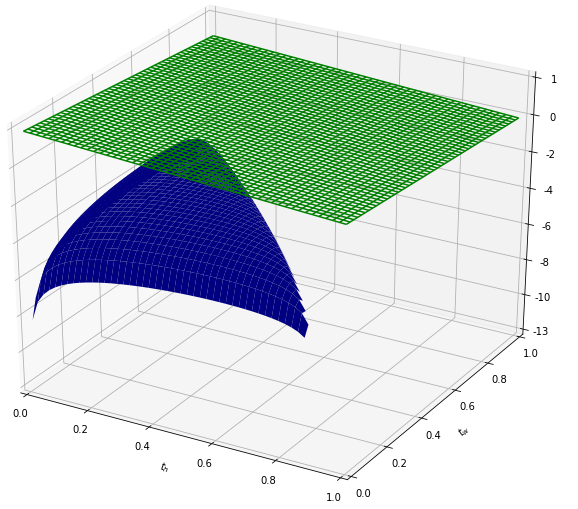
\includegraphics[width=0.48\textwidth]{plotNumericalExample01.png}}}%
%	\quad
%	\subfloat[The value of travel time as a function of $\alpha$]{{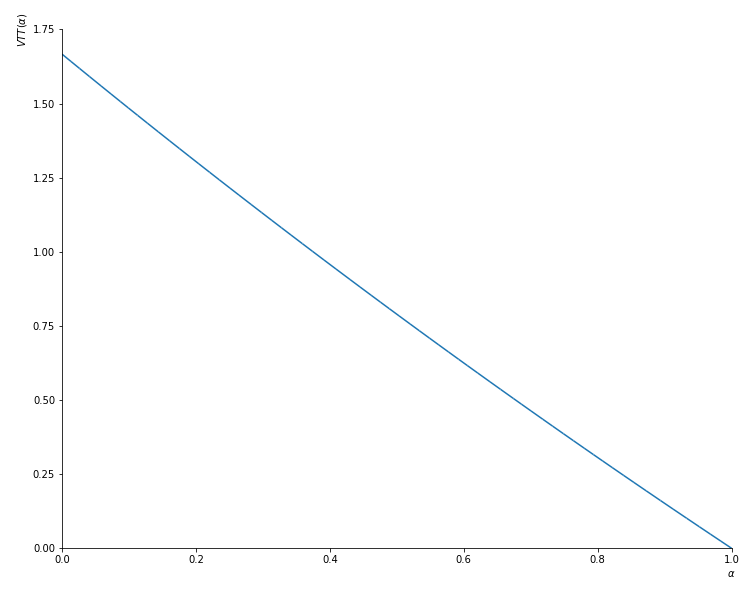
\includegraphics[width=0.48\textwidth]{plotNumericalExample02.png} }}%
%	\caption{Some features of the optimum}%
%	\label{fig:example}%
%\end{figure}






\section{The case with random travel times }

\subsection{The optimal allocation}

Suppose travel time $T$ is a random variable with a distribution bounded between $0$ and $Q$ \textit{such that the time constraint is never exceeded}.\footnote{\color{red}The trip is taken if the commuter expects that he or she will have some time at the destination to carry out the work-based activities. Hence, the travel time should be bounded within a reasonable limit for the trip to be taken. How can we put a bound to the distribution of travel time to take into account this?} We parametrise travel time in a convenient form $T=\mu+\sigma X$, where $\mu$ is its mean, $\sigma$ its standard deviation and $X$ is a standardised random variable with zero mean and unit variance and a probability density function $f\left(X\right)$.

Since utility depends on the unknown travel time, $T$, it is stochastic and hence the exact outcome for a given allocation of time cannot be determined before the trip. We assume the commuter allocates the total available time across different activities in view of a known travel time distribution. The choice of optimal time allocation is taken sequentially. Firstly, for a given travel duration and time assigned to the work-based activities, the commuter optimally allocates his or her time at home between the home-based and mobile activities. Once travel time is realised upon arrival at work, the commuter optimally allocates the remaining time between the work-based and mobile activities. We solve the utility maximisation problem by backward induction: Conditional on the information at the time of arrival at work, the commuter determines the optimal time to be assigned to the work-based activity given the realised travel time and the time devoted to the home-based and mobile activities. Then, the optimal time for the home-based activities is determined considering the distribution of travel times.

Upon arrival at the destination, the commuter has $Q-T-t_{d}$ time units to be allocated between the mobile and work-based activities.
As travel time is realised, the commuter faces no uncertainty and his/her problem amounts to:
\begin{align}
\begin{split}
\max_{t_{w}} \quad & U_{m}\left(t_{w} ; t_{h}, X \right) + U_{w}\left(t_{w}\right) \\
\mbox{subject to } \,\, & t_{w} \leq Q-\mu-\sigma X-t_{d} \\
 & t_w \geq 0
\end{split}
\label{eq:secondStageProb}
\end{align}
The constraint indicates that the time that will be allocated to the work-based activities cannot exceed the total available time at the
destination. The Lagrangian of the maximisation problem will be%
\begin{equation*}
U_{m}\left(t_{w}; t_{h}, X \right) + U_{w}\left( t_{w}\right)+\eta\left(Q-\mu-\sigma X-t_{d}-t_{w}\right),
\end{equation*}
with first-order conditions for an optimum being%
\begin{subequations}
	\label{eq:tw_stage}
	\begin{align}
	U_{w}^{\prime}\left(t_{w}\right) - U_{m}^{\prime}\left(t_{w}; t_{h}, X\right)-\eta & =0
	\label{eq:stage2_wrt_tw}\\
	\eta\left(Q-\mu-\sigma X-t_{d}-t_{w}\right) & =0\label{eq:stage2_compl}\\
	\eta,t_{w} & \geq 0
	\label{eq:stage2_nonnegative}
	\end{align}
\end{subequations}
If the commuter has a non-binding constraint, then the optimal time assigned to the work-based activity, $\hat{t}_{w}$, will be that which equates the value of time assigned to the work-based and mobile activities. If however the commuter faces binding constraint, then all the time at the destination will be assigned to the work-based activities, hence $\hat{t}_{w}=Q-t_{d}-\mu-\sigma X$. In this case, the value of time assigned to the work-based activities will be higher than that allocated to the mobile activity. This is so since, if this was not the case, then the commuter will be better off allocating some of the time at work to perform the mobile activities. If there exists a pair $\left(\hat{t}_{w},\hat{\eta}\right)$ satisfying the first-order conditions in (\ref{eq:tw_stage}), then the optimal utility at this stage is%
\begin{equation*}
V\left(\hat{t}_{w};t_{h}, X\right)\equiv U_{m}\left(\hat{t}_{w}; t_{h}, X\right) + U_{w}\left(\hat{t}_{w}\right).
\end{equation*} %
Note that, the time optimally assigned to the work-based activities, $\hat{t}_w(t_h)$, is defined for a given time assigned to the home-based activity, $t_h$. Given the optimal allocation of time at work, the commuter will determine the optimal allocation of the total time at the origin between the home-based and mobile activities. This decision is made in light of the travel time distribution as the exact travel time is not known before the trip. The commuter's problem then is to choose the time to be assigned to the home-based activities in order to maximise expected utility:
\begin{align}
\begin{split}
\max_{t_{h}} \quad & E\left[U_{h}\left(t_{h}\right)+V\left(\hat{t}_{w};t_{h}, X\right)\right]\\
\mbox{subject to } \,\, & t_{h} \leq t_{d} \\
& t_h \geq 0
\end{split}
\label{eq:firstStageProblem}
\end{align}
where the expectation is over all possible values of the standardised travel time, $X$. The Lagrangian of the utility maximisation problem can be given as:
\begin{equation*}
E\left[U_{h}\left(t_{h}\right) + V\left(\hat{t}_{w}; t_{h}, X \right) + \phi\left(t_{h} - t_{d} \right)\right]
\end{equation*}
with first-order conditions
\begin{subequations}\label{eq:th_stage}
\begin{align}
E\left[U_{h}^{\prime}\left(t_{h}\right) - U_{m}^{\prime}\left(t_{h} ,\hat{t}_{w}; X\right) - \phi\right] & =0
\label{eq:stage1_wrt_th}\\
\phi,t_{h} & \geq 0
\label{eq:stage1_lambda}\\
\phi\left(t_{d}-t_{h}\right) & =0
\label{eq:stage1_lambdai_const}
\end{align}
\end{subequations}
where $ \phi \geq 0 $. 
An optimal allocation exists if there is a quartet $\left(\hat{t}_{h}, \hat{t}_{w}, \hat{\eta},\hat{\phi}\right)$ satisfying the conditions in (\ref{eq:tw_stage}) and (\ref{eq:th_stage}). The existence and uniqueness of such an optimum is given in the following theorem:
\begin{theorem}
\label{thm:existence_stochastic}
Suppose each utility component is increasing, strictly concave and twice-continuously differentiable. Then, there exists a unique optimal time allocation, $\left(\hat{t}_{h},\hat{t}_{w}\right)$, and multipliers $\hat{\eta}$ and $\hat{\phi}$ satisfying (\ref{eq:tw_stage}) and (\ref{eq:th_stage}).
\end{theorem}


\begin{proof}
We want to show the existence of a unique quartet $\left( \hat{t}_{h},\hat{t}_{w}, \hat{\eta},\hat{\phi}\right)$ such that $\left( \hat{t}_{w}, \hat{\eta}\right)$ solves \eqref{eq:secondStageProb} given $\left( \hat{t}_{h},\hat{\phi}\right)$ and $\left( \hat{t}_{h},\hat{\phi}\right)$ solves \eqref{eq:firstStageProblem} given $\left( \hat{t}_{w},\hat{\eta}\right)$. The existence of a unique solution for each problem is given by the proof of Theorem \ref{thm:optimum_det}. The same proof establishes the existence of a unique joint solution if $V\left(\hat{t}_{w};t_{h}\right)$ is strictly concave in $t_{h}$. Since $V$ is continuous in $t_{h}$, strict concavity follows if $\frac{\partial}{\partial t_{h}}\left(\frac{\partial V}{\partial t_{h}}\right) \leq 0$. To see if this is the case, twice differentiate $V$ to find that%
\begin{equation*}
\frac{\partial}{\partial t_{h}}\left(\frac{\partial V}{\partial t_{h}}\right) = U_{m}^{\prime\prime} \left(t_{h}, \hat{t}_{w}; X \right) \left( 1 + \frac{\partial\hat{t}_{w}}{\partial t_{h}}\right)
\end{equation*}
So, strict concavity holds if $\frac{\partial\hat{t}_{w}}{\partial t_{h}} > -1$. Differentiating \eqref{eq:stage2_wrt_tw} and manipulating, we see that  $\frac{\partial\hat{t}_{w}} {\partial t_{h}} \geq 0$ and hence $V$ is strictly concave.
\end{proof}


The commuter chooses an optimal departure time given the choice of optimal allocation. This choice depends on the status of the two constraints: If the commuter has binding constraints at both ends of the trip, then $\hat{t}_{w}=Q-t_{d}-\mu-\sigma X$ and the mobile activity will be carried out only while travelling, hence $\hat{t}_{m}=\alpha\left(\mu+\sigma X\right)$. In this case, the expected marginal value of time assigned to the mobile activities will be lower than that allocated to the home-based or work-based activities. In addition, $\hat{t}_{h}=t_{d}$, hence the commuter will optimally depart as soon as he or she spent the last minute of the time allocated to the home-based activities. This is also the case with binding constraint at home irrespective of the status of the constraint at work.

On the other hand, if both the constraints are non-binding, then the marginal expected utility of time will be equalised across the three activities. This is analogous to the case with deterministic travel time. In this case, the optimal departure time can be any moment between $\hat{t}_{h}$ and $Q-\hat{t}_{w}-\mu-\sigma X$.\footnote{Since the exact travel time is unknown before the trip, the optimal departure time may be determined based on a predicted travel time such as the mean, median or other features of the travel time distribution.} This is also the case if the constraint at home is non-binding irrespective of the status of the constraint at work.

If the commuter has binding constraint at work but non-binding constraint at home, i.e., $\eta>0$ and $\phi=0$, then optimality requires that the expected marginal utility of time in the work-based activity be higher than that in the mobile or home-based activities. In this case, the optimal departure time can be any moment between $\hat{t}_{h}$ and $Q-\hat{t}_{w}-\mu-\sigma X$. Conversely, if the constraint at home is binding while that at work is not, the optimal departure time will coincide with the end of time assigned to the home-based activities. In this case, the expected marginal value of time devoted to the home-based activities will be higher than that allocated to the mobile or work-based activities.

The optimal expected utility:
\begin{equation*}
W\equiv E\left[U\left(\hat{t}_{h},\hat{t}_{w}; X\right)\right] = E\left[ U_{h}\left(\hat{t}_{h} \right) + U_{m}\left(\hat{t}_{h},\hat{t}_{w}; X\right) + U_{w}\left(\hat{t}_{w}\right)\right],
\end{equation*}
increases with the productivity of in-vehicle time, $\alpha$. Hence, as was the case with deterministic travel time, an improvement in the productivity of in-vehicle time is welfare improving.

% \subsection*{Example}

\subsection{Comparative statics}

\subsubsection*{The value of mean travel time}

% The value of (mean) travel time equals the expected difference in the value of time assigned to the work-based activity and that assigned to the mobile activity:
% The value of reduced mean travel time is the difference in the expected value of time assigned to the work-based activity and the expected value of in-vehicle time:
The value of reduced mean travel time is the sum of the resource value of time at work and the expected marginal benefit from undertaking the mobile activities at home/work rather than in-vehicle:
\begin{align}
-\frac{\mathrm{d}W}{\mathrm{d}\mu} & = E\left[ \left( 1 - \alpha\right) U_m^{\prime} \left(\hat{t}_{h}, \hat{t}_{w}; X \right) \right] + \hat{\eta}
\label{eq:VOT_stochastic}
\end{align}
Since $0\leq \alpha \leq 1$, $\hat{\eta}\geq 0$ and $U_{m}^{\prime} \left( \hat{t}_{h}, \hat{t}_{w}; X\right) \geq 0$, the value of travel time is non-negative. Substituting \eqref{eq:stage2_wrt_tw} in the above and rearranging, the value of travel time can be given by $E\left[ U_{w}^{\prime}\left( \hat{t}_{w} \right) - \alpha U_{m}^{\prime}\left(\hat{t}_{h}, \hat{t}_{w}; X\right)\right]$.  Notice that this is analogous to the expression for the value of travel time with deterministic travel time. Now, since travel time is uncertain, the the value of travel time is the \textit{expected} gain from using the saved travel time to perform the mobile activities at work rather than in-vehicle.

%We now examine the value of travel time with respect to the productivity of in-vehicle time for commuters with and without binding time constraints. 
If in-vehicle time is fully productive, i.e., $\alpha=1$,  then the value of travel time for commuters with non-binding constraints equals zero while those with binding constraints will have a positive value of travel time. This result is similar to the case with deterministic travel time. % and it indicates that ...

If the constraint at work is non-binding and travel time is fully productive, then the value of travel time will be zero. However, if the constraint is binding, then the value travel time will be positive even if travel time is fully productive. This result is also similar to the case with deterministic travel time.

\begin{prop}
The value of travel time declines with an exogenous improvement in the productivity of in-vehicle time if the constraints are non-binding; or the coefficient of relative risk aversion of $U_m$ is less than or equal to unity should the constraints be binding.
\end{prop}

\begin{proof}
	
	Differentiating (\ref{eq:tw_stage}) and (\ref{eq:th_stage}) with respect to $\alpha$ and rearranging, we observe that $\frac{\partial\hat{t}_{h}}{\partial\alpha} \geq 0$ and $\frac{\partial\hat{t}_{w}}{\partial\alpha}\geq0$. In particular, if the constraints are non-binding, then $\frac{\partial\hat{\eta}}{\partial\alpha}=0 $ and
	\begin{equation*}
	\frac{\partial\left(-\frac{\mathrm{d}W}{\mathrm{d}\mu}\right)}{\partial\alpha} = E\left[\left(1-\alpha\right)  \left( \mu + \sigma X \right) \left(\frac{\prod_{i \in\left\{ h, m, w \right\}}U_{i}^{\prime\prime}\left(\hat{t}_{i}\right)}{\sum_{i\neq j}U_{i}^{\prime\prime}\left(\hat{t}_{i}\right)U_{j}^{\prime\prime}\left(\hat{t}_{j}\right)}\right)-U_{m}^{\prime}\left(\hat{t}_{h}, \hat{t}_{w}; X\right)\right] \leq 0
	\end{equation*}
	where the inequality follows since $0 \leq \alpha \leq 1$ and $U^{\prime\prime}_i < 0 < U^{\prime}_i$.  If the constraints are binding, then $\frac{\partial\hat{t}_{h}}{\partial\alpha}=\frac{\partial\hat{t}_{w}}{\partial\alpha}=0$, $\hat{t}_{m}=\alpha \mu + \sigma X$ and $\frac{\partial\hat{\eta}}{\partial\alpha}=-(\mu+\sigma X) U_{m}^{\prime\prime}\left(\alpha (\mu+\sigma X) \right)$. Therefore,
	\begin{equation*}
	\frac{\partial\left(-\frac{\mathrm{d}W}{\mathrm{d} \mu}\right)}{\partial\alpha}= E\left[-\alpha (\mu + \sigma X) U_{m}^{\prime\prime}\left(\alpha (\mu+\sigma X) \right)-U_{m}^{\prime}\left(\alpha (\mu+\sigma X) \right)\right] \leq 0
	\end{equation*}
	if $\frac{-\alpha (\mu+\sigma X) U_m^{\prime\prime} \left(\alpha (\mu+\sigma X)\right)}{U_m^{\prime\prime} \left(\alpha (\mu+\sigma X)\right)} \leq 1$ as claimed.\footnote{\color{red}Alternatively, 
		\begin{equation*}
			\frac{\partial\left(-\frac{\mathrm{d}W}{\mathrm{d}\mu}\right)}{\partial\alpha}=E\left[U_{w}^{\prime\prime}\left(\hat{t}_{w}\right)\frac{\partial\hat{t}_{w}}{\partial\alpha}-U_{m}^{\prime}\left(\hat{t}_{h},\hat{t}_{w};X\right)-\alpha\left(\mu+\sigma X-\frac{\partial\hat{t}_{h}}{\partial\alpha}-\frac{\partial\hat{t}_{w}}{\partial\alpha}\right)U_{m}^{\prime\prime}\left(\hat{t}_{h},\hat{t}_{w};X\right)\right]
		\end{equation*}
		Thus,  $\frac{\partial\left( -\frac{\mathrm{d}W} {\mathrm{d}\mu}\right)} {\partial\alpha} \leq 0$ if $ E\left[-U_{m}^{\prime}\left(\hat{t}_{h},\hat{t}_{w};X\right)-\alpha\left(\mu+\sigma X\right)U_{m}^{\prime\prime}\left(\hat{t}_{h},\hat{t}_{w};X\right)\right] \leq 0$ or $-\frac{\alpha\left(\mu+\sigma X\right)U_{m}^{\prime\prime}\left(\hat{t}_{h},\hat{t}_{w};X\right)}{U_{m}^{\prime}\left(\hat{t}_{h},\hat{t}_{w};X\right)} \leq 1$
	}

\end{proof}


As was the case with deterministic travel duration, the result stated in the above proposition implies that lower value is  attached to reduced travel time as productivity enhancing technologies continue to improve. As was the case with deterministic travel duration, the result stated in the above proposition implies individuals attach more value for an improvement in productivity enhancing technologies during the transition period than once the technology is matured.  

As was the case with deterministic travel duration, the result stated in the above proposition implies individuals attach more value for an improvement in productivity enhancing technologies during the transition period than once the technology is matured.  


\subsubsection*{The value of reliability}

The value of reliability in our model is:
\begin{align*}
-\frac{\mathrm{d}W}{\mathrm{d}\sigma} & = E\left[\left( 1 - \alpha \right) X U_{m}^{\prime} \left(\hat{t}_{h}, \hat{t}_{w}; X\right)\right],
\end{align*} %
which is proportional to $1-\alpha$.\footnote{This has been indicated by {\color{blue}Fosgerau (2017)} in an ITF Roundtable discussion paper} As stated in the following lemma, the value of reliability is non-negative implying that the commuter is willing-to-pay a certain amount for a reduction in the degree of travel time variability.

\begin{lemma}
An exogenous reduction in travel time variability is beneficial to the commuter, i.e., the value of reliability is non-negative.
\end{lemma}

\begin{proof}
Let $ v_1 $ and $v_2$ respectively denote the value of $U_{m}^{\prime}\left(\hat{t}_{h}, \hat{t}_{w}; X\right)$ for $ X > 0$ and $X \leq 0$, where $v_{1}$ and $v_{2}$ are positive constants with $v_{1}\geq v_{2}$ since $\frac{\partial U_{m}^{\prime} \left(\hat{t}_{m}\right)}{\partial X} \geq 0$. Using this, the value of reliability can be given as\footnote{Consider weighting by the probability of positive and negative values of $X$.}
\begin{align*}
-\frac{\mathrm{d}W}{\mathrm{d}\sigma} & = E\left[\left(1-\alpha\right) X U_{m}^{\prime} \left(\hat{t}_{h}, \hat{t}_{w}; X\right)\vert X>0\right]  + E\left[\left( 1 - \alpha \right) X U_{m}^{\prime}\left( \hat{t}_{h}, \hat{t}_{w}; X\right) \vert X\leq 0 \right] \\
 & = E\left[\left( 1 - \alpha \right) v_{1} X \vert X > 0 \right] + E\left[\left( 1 - \alpha \right) v_{2} X \vert X \leq 0 \right]
 \end{align*}%
Noting that $E\left[X\right]=0$ such that $E\left[X \vert X \leq 0 \right] = -E\left[ X \vert X > 0 \right]$, we have%
\begin{align*}
- \frac{\mathrm{d}W}{\mathrm{d}\sigma} & = \left(1-\alpha\right) v_{1} E\left[X\vert X > 0 \right] + \left(1-\alpha \right) v_{2} E\left[X \vert X\leq0\right]\\
 & =\left(1-\alpha\right)v_{1}E\left[X\vert X>0\right]-\left(1-\alpha\right)v_{2}E\left[X\vert X>0\right]\\
 & =\left(1-\alpha\right)\left(v_{1}-v_{2}\right)E\left[X\vert X>0\right]\\
 & \geq0
\end{align*}
where the inequality follows since $v_{1}\geq v_{2}$ and $E\left[X\vert X>0\right] > 0$. Therefore, the value of reliability is non-negative.
\end{proof}

Notice that the value of reliability equals the weighted mean of gains from undertaking the mobile activity at work instead of while travelling. Thus, if in-vehicle time is as productive as time at work, i.e., $\alpha=1$, then the commuter does not gain by using the reduced travel time to carry out the mobile activity at work. Hence, the value of reliability will be zero if in-vehicle time is fully productive. This is new compared to previous literature \citep{Small1982SchedulingConsumerActivities,FosgerauEngelson2011ValueTravelTime,FosgerauKarlstroem2010ValueReliability} who


\todo[inline]{Compare the value of reliability in our model against that in \citet{FosgerauEngelson2011ValueTravelTime}, where $ \beta, \gamma <0 $ shall be assumed so their result can be comparable to ours}

\todo[inline]{Note: The following need revision as it does not hold in general, and it proved to be difficult to come up with a conditon that ensures the inequality holds}

\begin{prop}
	WRONG !!!
The value of reliability declines with an exogenous increase in the productivity of in-vehicle time provided that both constraints are binding or non-binding.
\end{prop}

\begin{proof}
If both constraints are non-binding, then $\hat{\eta}=\hat{\phi}=0$ and hence
\begin{align*}
\frac{\partial\left(-\frac{\mathrm{d}W}{\mathrm{d}\sigma}\right)}{\partial\alpha} &= E\left[\left(\left(1-\alpha\right)\left(\mu+\sigma X\right) \frac{\prod_{i \in \left\{ h,w,m\right\}  }U_{i}^{\prime\prime}\left(\hat{t}_{i}\right)}{\sum_{i\neq j}U_{i}^{\prime\prime}\left(\hat{t}_{i}\right)U_{j}^{\prime\prime}\left(\hat{t}_{j}\right)}-U_{m}^{\prime}\left(\hat{t}_{m}\right)\right)X\right] \leq 0
\end{align*}
where the inequality follows since the expression in parenthesis is negative. If the constraints are binding, then $\frac{\partial\hat{t}_{h}}{\partial\alpha}=\frac{\partial\hat{t}_{w}}{\partial\alpha}=0$, and hence $\frac{\partial\hat{t}_{m}}{\partial\alpha}=\mu+\sigma X$ and
\begin{equation*}
\frac{\partial\left(-\frac{\mathrm{d}W}{\mathrm{d}\sigma}\right)}{\partial\alpha}=E\left[\left(\left(1-\alpha\right)\left(\mu+\sigma X\right)U_{m}^{\prime\prime}\left(\hat{t}_{m}\right)-U_{m}^{\prime}\left(\hat{t}_{m}\right)\right)X\right] \leq 0.
\end{equation*}
Therefore, $\frac{\partial\left(-\frac{\mathrm{d}W}{\mathrm{d}\sigma}\right)}{\partial\alpha} \leq 0 $ irrespective of whether the constraints are binding.
\end{proof}

An increase in the productivity of in-vehicle time reduces the $\left(1-\alpha\right)$ and hence also the value of reliability, but its effect through $t_{m}$ depends on if and how much the optimal allocation of time changes due to a change in $\alpha$. With binding time constraints at both ends of the trip, $\frac{\partial t_{m}}{\partial\alpha}=\mu+\sigma X>0$ since the time optimally allocated to the home-based and work-based activities will remain unchanged. Thus, the value of reliability declines with the productivity of in-vehicle time irrespective of the value of $\frac{\partial t_{m}}{\partial\alpha}$. However, when one or both constraints are inactive, a change in productivity of in-vehicle time also affects the value of reliability through its effect on the optimal allocation of time. Accordingly, an increase in $\alpha$ increases $t_{h}$ or $t_{w}$ or both. As a result, the value of reliability declines with the productivity of in-vehicle time only if the sum of the change in time devoted to the home-based and work-based activities does not exceed the travel time, i.e., $\frac{\partial\hat{t}_{h}}{\partial\alpha}+\frac{\partial\hat{t}_{w}}{\partial\alpha}\leq\mu+\sigma X$.


\section{Conclusion and policy implications}

The model examines the optimal allocation of time among different activities and the valuation of travel time and reliability with self-driving cars. It analyses how the values of travel time and reliability changes with increased productivity of in-vehicle time.

\clearpage

% \bibliographystyle{authordate1}
\bibliographystyle{chicago}
\bibliography{references}

\end{document}

